
\documentclass[apj]{emulateapj}

\usepackage{graphicx}
\usepackage{amssymb}
\usepackage{amsmath}
\usepackage{natbib}
\bibliographystyle{apj}
\usepackage[breaklinks,colorlinks,citecolor=blue,linkcolor=magenta]{hyperref}
\shortauthors{Zhou et al.}

%%% new command %%%
\newcommand{\ima}{\texttt{ima} files }
\newcommand{\flt}{\texttt{flt} files }
\newcommand{\eps}{$\mathrm{e}^{-}/\mathrm{s}$}
\newcommand{\tinytim}{\textit{Tiny Tim}}
\newcommand{\bpic}{$\beta$ Pic}
\newcommand{\vsini}{$v\sin i$}
\newcommand{\mjup}{M$_{\mbox{Jup}}$}
\begin{document}

\title{Variability of Planetary Mass Companion 2M1207 B}
\shorttitle{Variability of 2M1207 B}
\author{Yifan Zhou, Daniel Apai, Glenn Schneider, ...}
\affil{The University of Arizona}

\begin{abstract} Rotational modulations in disk-integrated light of
brown dwarfs have recently provided powerful constraints on the
properties of ultracool atmospheres, including longitudinal and
vertical cloud structures and cloud evolution. Furthermore, detection
of periodic light curve variations can directly probe the rotational
periods of ultracool objects.

We present here, for the first time, time-resolved high-precision
photometric measurements of a planetary-mass companion, 2MASS1207b, to
a brown dwarf primary. Using HST/WFC3 and point spread function %in
combination with two spacecraft roll angles we detect photometric
modulations in the light curve. The amplitude is 0.9\% in the F160W
and 1.5\% in the F125W filters; we find a consistent period and
similar phase in both bands. Joint fit to the lightcurve in both bands
suggest a period of $10.2^{+0.9}_{-0.8}$ h. The relative amplitudes in the two
filters are very similar to that found in a recent study of a field
(high-gravity) L-dwarf, suggesting that the cloud structures that
introduce the photometric modulations are similar in high- and
low-gravity objects. Importantly, our study also measures, for the
first time, the rotational period for directly imaged planetary-mass
companion.
\end{abstract}

\keywords{brown dwarfs -- planets and satellites: atmospheres -- planets
  and satellites: individual (2M1207b) -- techniques: photometric}
\maketitle
%
\section{Introduction}

Cloud properties in high- and low-gravity objects -- thick clouds: an
explanation for very red and faint near-infrared fluxes of directly
imaged planets

Rotational mapping is powerful: successes in brown dwarfs...

The target 2M1207b... contrast The key challenge of obtaining the
lightcurve of 2M1207b is the high contrast to and small separation
from 2M1207A.


In this Letter we present the first high-contrast, high-precision,
time-resolved observations of a directly imaged planet or
planetary-mass object. We successfully detect rotational modulation
and measure the amplitudes in two bands and determine the rotational
period.

\section{Observation} We obtained direct images of the 2M1207A+b
system on UT 2014 April 11from 08:07:47 to 16:53:18 using the Hubble
Space Telescope (HST) and its Wide Field Camera 3 \citep[WFC3,
][]{Kimble2008} in the frame of the HST Proposal GO-13418 (PI:
D. Apai). We acquired the observations in filters F125W
($\lambda_{\mbox{pivot}}$ = 1245.9 nm, full width at half maximum
(FWHM) = 301.5 nm) and F160W ($\lambda_{\mbox{pivot}}$ 1540.52, FWHM =
287.9 nm), roughly corresponding to the J and H bands. The WFC3 pixel
scale is $\approx$13mas. We used the $256\times256$ pixels sub-array
mode to avoid memory dumps during the observations.  In order to
provide a near-continuous coverage for detecting modulations we
observed the 2M1207 system in six consecutive HST orbits, obtaining
data with cadence of $\sim1.5$ minutes over a baseline of 8 hours and
40 minutes. The observations were interrupted by 58 minute-long Earth
occultations every 94 minutes.

The observations applied space craft rolls between each two orbits to
allow roll-subtraction of the primary \citep[e.g.][]{Song2006}. The
telescope roll angles for orbits 1, 3, and 5, and those taken in
orbits 2, 4, and 6 differed by $25^{\circ}$. At the separation of
2M1207b this angle difference corresponds to a displacement of
$0.34''$ or 2.75 and 2.30 resolution elements in F125W and F160W,
respectively. In each orbit we took thirteen SPARS10 non-destructive
read-outs with NSAMP=10, alternating between F160W and F125W filters,
with 2--3 identical exposures in one exposure sequence. To improve PSF
sampling and reduce the risk caused by bad pixels, we applied standard
4 point dithering. Over the 6 orbits, we obtained 70 images with 10
non-destructive read-outs in F125W and 64 images in F160W with
exposure time of 88.4~s in each filters.

\section{Data Reduction}

%Although \cite{Mandell2013} stated that WFC3 IR time series
%extract from {\flt} have a rms 1.3 times larger than that obtained
%from {\ima}, \flt keeps all pixels of the image of 2M1207 A
%unsaturated, while in 80\% of non-destructive reads the cores of
%2M1207 A are saturated. 
%Thus \flt help better align the images for
%primary subtraction, and separate the flux of 2M1207 B from that of
%2M1207A.


%The small angular separation of 2M1207 A and B (as shown in Figure
%\ref{fig:1}) makes precise primary star subtraction and photometry
%very difficult. 
%On the under-sampled WFC3 IR detector (plate scale
  %$\sim 0.13''\mbox{pixel}^{-1}$ \cite{dressel2012wide}), the primary
%and the secondary only separate by $\sim 6$ pixels, which is about 5
%times of the FWHM of the PSF. In addition, under-sampling causes
%significant artifacts when shifting the images for registration no
%matter what interpolation method is used.

\begin{figure*}
  \centering
  \plottwo{original}{subtracted}
  \caption{WFC3 F160W images of 2M1207A system. {\em Upper panel}: In the original image 
    2M1207 B is hidden in the halo of the bright 2M1207A.   {\em Lower panel:} In the residual image -- after the subtraction of the hybrid PSF -- 2M1207 B is detected at a high significant level.}
  \label{fig:1}
\end{figure*}

\subsection{Photometry}

We started the reduction from the the \flt files produced by the
WFC3's \texttt{calwfc3} pipeline. We did not opt to use the more
advance \ima pipeline products because these provided less information
on 2M1207A, which saturated after the first few read-outs.  The \flt
are results of basic calibration, including dark current correction,
non-linearity correction, flat field correction, as well as
up-the-ramp fit on the non-destructive read-outs also considering
cosmic rays. From the beginning, pixels with data quality flags ``bad
detector pixels'' (DQ = 4), ``unstable response'' (DQ = 32), and ``bad
or uncertain flat value'' (DQ = 512) were masked out and excluded from
further analysis as suggested by previous transit exoplanet
spectroscopic observations\citep[e.g.][]{Berta2012, Kreidberg2014}.


One major challenge of high contrast imaging observation using WFC3/IR
is significant under-sampling of the detector.  2M1207 A and b are
only separated by $\sim6$ pixels or $\sim$5 FWHM of the PSF. When
applying roll subtraction, notable artifact structures are generated
by image interpolation and shifting. On the other hand, \tinytim{} PSF
simulator\citep{Krist1995} offers a solution by providing Nyquist
sampled PSF, but significant systematic errors of \tinytim{} PSF
 limits its ability in high precision
photometry\citep{Biretta2014}. However, 6 orbits of observation
provides us an opportunity to
fully characterize the difference of model and observed PSFs. To obtain
robust \tinytim{} PSF photometry,  we designed a 2-round PSF fitting strategy: 1. calculating
correction map for \tinytim{}; 2. hybrid PSF photometry.

For both of 2 rounds, we used {\em Tiny Tim} to calculate 10$\times$
over-sampled model PSFs based the filters, the spectra 
\citep{Bonnefoy2014, Patience2010}, the telescope's actual focus, and
the telescope jitter.  We used the new set of Tiny Tim parameters
provided by \cite{Biretta2014} to better model the cold mask,
diffraction spikes, and the coma. The focus parameters were calculated
using the model listed on the STScI
website\footnote{\url{http://www.stsci.edu/hst/observatory/focus/FocusModel}}.
We determined the exact position of 2M1207A first by fitting the PSF
on a dynamic coordinate grid and minimizing the difference in the
observed and modeled PSFs at a region centered on 2M1207 A with a
5-pixel-radius aperture centered on 2M1207 b excluded. Then introduce
another \tinytim{} PSF for 2M1207b and  fit the
position of 2M1207 b and the photometries of 2M1207 A and b together
by least square optimization. From our data set, we discovered that
the difference of observed PSFs and model PSFs are very stable for
given PSF position. Therefore at the end of the first round PSF
fitting, we derived 8 (2 roll angles $\times$ 4 dithering positions)
empirical correction maps for each filter:
\begin{equation}
  \mathrm{Corr = Median(PSF_{model} - PSF_{obs} )}
\end{equation}
where $\mathrm{PSF_{model}}$ is a combination of two \tinytim{} PSFs
for 2M1207 A and b. In the second round, we combined the correction
term linearly with the two \tinytim{} PSFs to generate hybrid PSFs,
and scaled the three component together to get best fit. We found that by including the correction term,
the reduced $\chi^{2}$ of PSF fitting is decreased from $\sim 10$ to
around unity. Because the total fluxes of the model PSFs were
normalized to unity as default, the fluxes of 2M1207 A and B were
solely represented by the amplitude of the two PSFs.

However, PSF profiles change with different exposure positions due to
pixelation, especially for the case that WFC3 IR is significantly
under-sampled. Also, the flat fields may potentially have large scale
structures \citep{dressel2012wide}. Because of these factors, the
fluxes for both 2M1207 A and B are correlated with the dithering
position. To break the correlation, we normalize each group of
exposures that have the same dithering position and roll angle
individually -- we took the median of the fluxes that were measured
from these exposures as normalization factors and devided them from
every photometric measurement. Because the normalization factor for
each group of exposures is calculated across the whole observation,
this normalization step have negligible impacts on variability
analysis.

% {\em Hybrid PSF Calculation:} The hybrid PSFs were generated as a
% linear combination of a diffraction-limited PSF (calculated with the
% {\em Tiny Tim} simulator\citep{Krist1995}, and a empirically
% determined correction map. We used {\em Tiny Tim} to calculate model
% PSFs for the filters used, the spectrum of our target, the telescope's
% actual focus, and the telescope jitter.  We used the new set of Tiny
% Tim parameters provided by \cite{Biretta2014} to better model the cold
% mask, diffraction spikes, and the coma. The focus parameters were
% calculated using the model listed on the STScI
% website\footnote{\url{http://www.stsci.edu/hst/observatory/focus/FocusModel}}.
% A significant advantage of Tiny Tim PSF over empirical PSFs is that
% Tiny Tim can produce Nyquist-sampled results, which allows accurate
% image shifting and interpolation. However, an important limitation of
% Tiny Tim is that the model PSFs have significant systematic
% errors. \cite{Biretta2014} demonstrated that the diffraction spikes
% and coma are not accurately simulated with Tiny Tim for WFC3/IR
% images. However, using the 6-orbit long time series, we are able to
% accurately characterize the difference of the modeled and observed
% PSFs and derive an empirical correction map: Corr = Mean (
% PSF\_modeled - PSF\_observed ) where PSF\_modeled is a combination of
% two Tiny Tim PSFs with positions and amplitudes optimized to minimize
% the residuals.  By combining the model PSFs with the empirical
% correction map we derived a high-quality hybrid PSF, the use of which
% significantly improved the PSF subtraction and photometry.

% {\em PSF Fitting:} In the next step we simultaneously fitted the positions and amplitudes of the combination of the hybrid PSFs to 2M1207A and 2M1207b. First, we determined the primary star position and telescope jitter. We produced a list of 10$\times$ over-sampled PSFs matching the spectrum \citep{Bonnefoy2014} and the position of 2M1207A with different telescope jitters ranging from 0 to 50$\mbox{mini-arcsec s}^{-1}$ along
% both $x$ and $y$ detector axes. The PSFs were registered with the original image by searching on a dynamic grid and minimizing the difference in the observed and modeled PSFs at a region centered on 2M1207 A with a 5-pixel-radius aperture centered 2M1207 B excluded. 

% Next, we determined the position and approximate flux of 2M1207B by calculating and fitting a Tiny Tim PSF for the hybrid PSF-subtracted 2M1207 B based on its position on the detector, spectrum \citep{Patience2010}, and
% the telescope jitter that had been obtained above. In the final step,
% we combined the two PSFs together. 

% We fixed the position of the primary as it had been fitted in the first step and fitted for the
% amplitudes of the two PSFs and the precise position of the
% secondary. Since the total fluxes of the model PSFs were normalized to
% unity as default, the fluxes of 2M1207 A and B were solely represented
% by the amplitude of the two PSFs coordinately.

% Because of the systematic errors of the Tiny Tim PSF, the quality of the
% fit is not perfect. The reduced $\chi^{2}$ values were at level
% of $\sim10$. However, we found that the residual patterns were very
% stable among the image that have the same dithering position and
% telescope rolling. Therefore, we median combined the residual images
% that have the same dithering position and telescope rolling angle to
% construct 8 residual models (4 dithering position $\times$ 2 telescope
% rolling angle) for each filter. We pre-subtract the corresponding
% residual from the original image and repeated the procedure that
% listed above. Using this extra-step, the reduced $\chi^{2}$
% greatly decreased to around unity.




% %\section{Uncertainty analysis}

\subsection{Uncertainty Analysis: White noise}
We consider the primary source of uncertainty for every measurement is
photon noise. We propagated the photon noises of every single pixel
that were calculated from count rates and detector gain, to the PSF
fitting results. The photon noises for photometry in F125W and F160W
are 1.33\% and 1.02\%, respectively.

Since the primary and secondary PSFs were fitted simultaneously in our
PSF photometry procedure, the uncertainties of photometry and position
for the primary and secondary are coupled with each other. The second
order uncertainty could also contribute to the overall uncertainty,
e.g. the imperfection of position measurement of 2M1207A can affect
the photometry of 2M1207b. We used a Monte Carlo (MC) method to evaluate the complete systematic of the
PSF fitting. We applied the PSF photometry to images that
were added with random Poisson noise and repeat the procedure for 1000
time. From the distribution of the result, the uncertainty for F125W
and F160W photometry are found to be 1.34\% and 1.12\%,
respectively. We conclude that the white noise of our observation is
dominated by photon noise. 

\subsection{Uncertainty Analysis: Flat field uncertainties}

 \begin{figure*}
  \centering
  \plotone{systematics}
  \caption{F125W (left) and F160W (right) light curves under different
  variability verification tests. Individual measurements are plotted with gray
  crosses. Photometries of the same exposure sequence are binned, and
  binned data are plotted with points or squares. Fitted sinusoidal
  waves are plotted with solid lines. {\em Upper}: binned photometries taken
in dithering position 1 and 3 (red points) and that taken in 2 and 4
(blue squares) are plotted differently. They demonstrate same trend of
variation. In upper left panel, sinusoidal wave fitted with all
parameter set free, and that fitted with period set the same as that
of F125W are plotted with green and purple lines, respectively. {\em
  Middle}: sinusoidal waves fitted without using the data taken in
Orbit 1 are plotted. These curves are almost identical to the curves
plotted in upper panel. {\em Lower}: photometry measured with
AFEM-applied images and their best fitted sinusoidal curves are
plotted. These photometries and curves are also almost identical to
those plotted in upper panel.}
  \label{fig:2}
\end{figure*}

In our observations 2M1207 B were observed at 8 different spots on the
detector (2 rolls $\times$ 4 dithering positions). Imperfect flat
field correction are potential sources of variation as they may
introduce position-dependent differences in the count rates. The
uncertainty of WFC3 IR pipeline flat field is $\sim 1\%$
\citep{dressel2012wide}.
% and our time resolved observations for another target
%demonstrate that aperture photometry for exposures taken at different
%dithering position are uncertain at the same level.
%Flat field uncertainties have smaller effects on 
In PSF photometry, however, multiple pixels are fitted simultaneously
and we expect a lower than 1\% uncertainty from the flat field
errors. To verify this we multiplied every image by an artificial flat
field error mask (AFEM) -- a uniformly distributed Gaussian noise array with
mean of 1 and sigma of 1\% -- and repeated the PSF photometry on the
resulting images.  The analysis of these experiments showed almost
identical lightcurve to the original, verifying that the flat field
errors do not affect our photometry significantly (Figure
\ref{fig:2}).


  \begin{figure*}
  \centering
  \plotone{sineCurveFit_binCombined}
  \caption{Normalized light curves for 2M1207 B (upper) and A (lower)
    with filter F125W (left) and F160W (right). Individual photometric
  measurement are plotted in gray crosses and binned photometry are
  plotted with red points. Best fitted sinusoidal waves are plotted
  with blue solid lines.}
  \label{fig:3}
\end{figure*}

\section{Verification of Photometric Variations and Amplitude
  Estimate}

\subsection{Tests and Verification}

The light curves that resulted from our photometry show apparently
sinusoidal modulations, discussed in more details in
\S,\ref{Results}. To verify that these modulations are intrinsic to
the object and not result of our data reduction procedure or due to
instrumental changes, we carried out three different tests.

First, we fitted sine waves independently to the two filters to verify
the similarity of the signal in the two bands (Figure \ref{fig:2}). Inconsistent periods or
light curve shapes would argue against a genuine signal.  We found
that the periods of the best fit sine waves are similar,
$10.5^{+1.2}_{-1.3}$h for F125W and $9.1^{+1.1}_{-1.0}$h for
F160W. These periods are roughly consistent within the
uncertainty. Furthermore, these periods are not close to any
timescales over which HST or WFC3 are known to changes.

 As a second test we repeated the analysis neglecting the first
 orbit. The motivation behind this test was that, due to spacecraft
 thermal settling, the first orbit of HST observations is often
 slightly unstable and is often neglected in high-precision studies
 (\textbf{citation?}). Indeed, in our analysis 2M1207 A is
 significantly fainter in the first orbit (Figure \ref{fig:3}) than in
 the subsequent ones.
 %The exposure levels at the pixels of the peak of the PSF of 2M1207 B are less than 10,000 e$^{-}$
 %for both two colors, thus image persistence is less of an issue for
 %2M1207 B. 
 Our analysis based on orbits 2--6 only found essentially identical
 results to our analysis of orbits 1--6, based on which we conclude
 that the first less reliable orbit does not affect our results
 significantly (Figure \ref{fig:2}, middle panel).

As a third test we explored whether a subset of images, perhaps
imperfectly normalized or correlated with specific instrument states,
could be driving the light curves into an apparently sinusoidal
shape. To test this possibility we split the data into two temporally
overlapping halves: sub-dataset one from dithering positions 1 and 3,
and sub-dataset two from dithering positions 2 and 4. For both
datasets we repeated our analysis independently.  For both of F125W
and F160W, two halves demonstrated similar trend of variability as
shown in Figure \ref{fig:2}.  Our analysis detected sinusoidal
modulations in {\em both} sub-datasets and in {\em both} filters, with
periods and amplitudes consistent with those derived from the complete
data set (\ref{fig:2}, upper panel).
 
 These tests demonstrate that the modulation seen in our data are
 consistently present in the different filters, in the different time
 segments of the data, and in data obtained in different dithering
 positions.
 



 % \begin{itemize}
% \item the source of the scattering -- 
% \item flat field uncertainty -- adding artificial flat field error mask
% \item validity of the variability\\
%   -- both filter demonstrate similar period of variability\\
%   -- split the data into two half, the trend in two halves of data
%   looks similar.
%   -- fix the position does not change the light curve
% \item uncertainty of sinusoidal curve fit
%   -- carry out a mcmc fit? is it worth doing this.
% \end{itemize}



\subsection{Amplitude and Period Measurements}

To constrain the uncertainties of the least square optimization
results, we used a MC method to improve the fitting. We
generated a series of random Gaussian noises with the standard deviation same as
the photon noise, added them to the original light curves, and applied
least square fit to the new light curves. We repeated above routine for 100,000 times and obtained
the distribution of the fitting parameters. The distributions for the
periods and the amplitudes for F125W and F160W light curves are
shown in Figure \ref{fig:4}.


\begin{figure*}
  \centering
  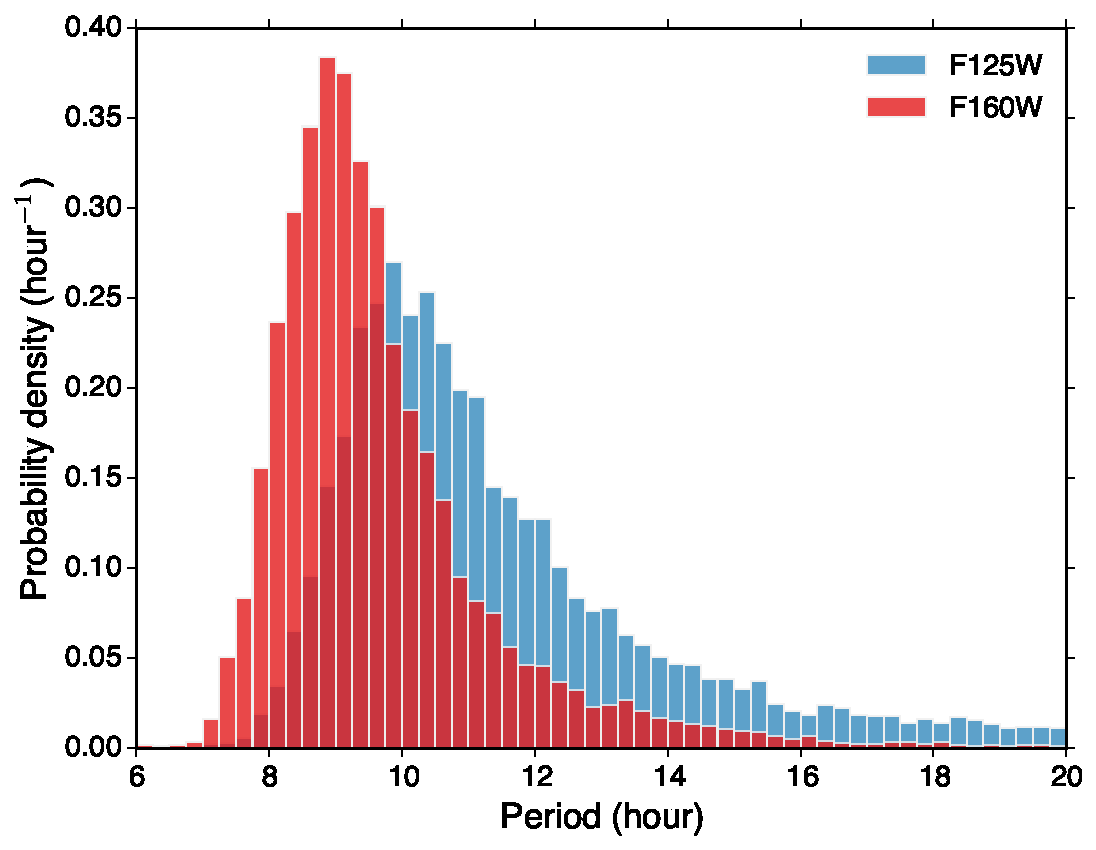
\includegraphics[width=0.45\textwidth]{periodDistr}
  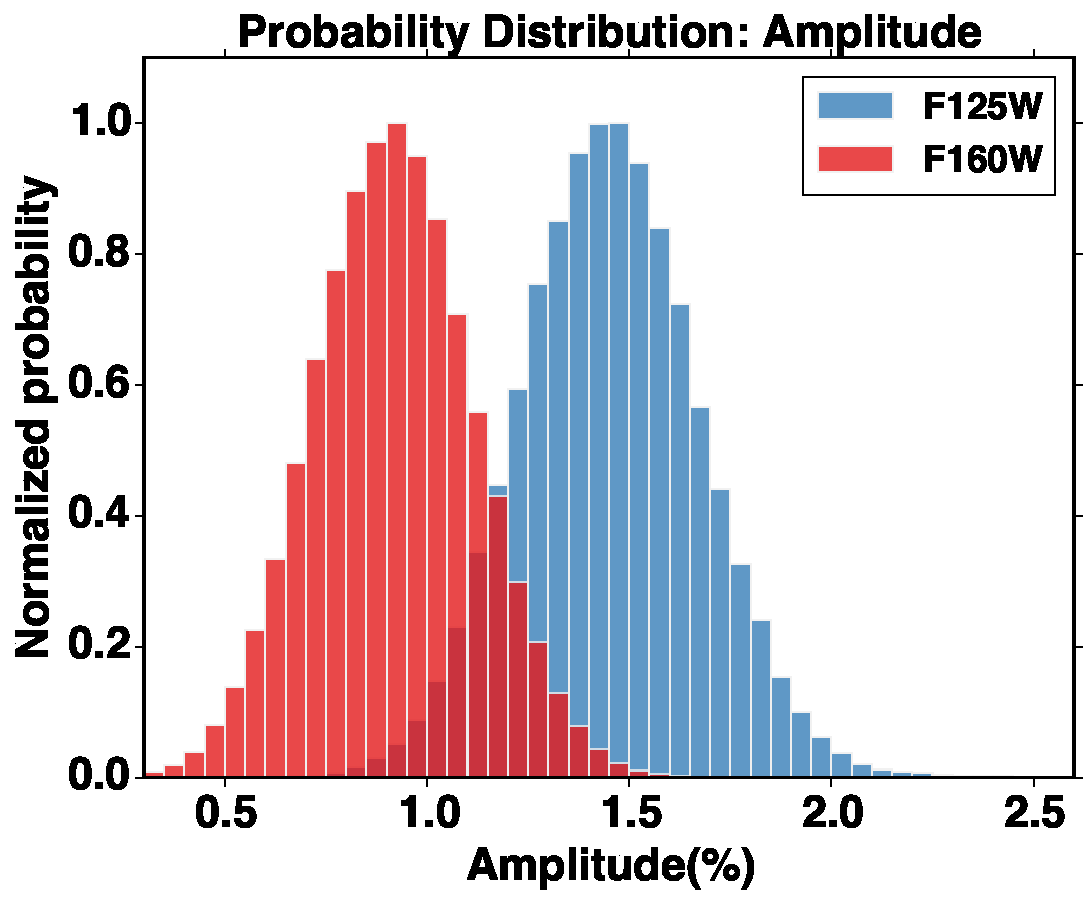
\includegraphics[width=0.45\textwidth]{amplitudeDistr}
  \caption{Distributions for periods (left) and amplitudes(right) for the light
    curve of F125W and F160W. The bin size for histograms of period is
  0.25 hour and for that of amplitude is 0.5\%. Histograms are
  normalized in the way that total area of the histogram equals to
  1. In the right panel, Gaussian profiles are fitted to the
  histograms of periods and plotted in solid lines.}
  \label{fig:4}
\end{figure*}

\section{Result}



\label{Results}
We present the first high-contrast, high-resolution, high-cadence, and
high-precision photometry of a directly imaged planet or
planetary-mass companion. Our observations reveal a modulation in the
light curve of the 5--7~M$_{J}$ companion 2M1207b, the first detection
of modulations in directly imaged ultracool objects.  The best fit
periods for F125W and F160W are 10.5 and 9.1 hour correspondingly. The
amplitudes for the normalized light curves are 1.45\% and 0.92\% for
F125W and F160W light curves. 

We obtained high signal to noise photometry series for both 2M1207 A
and B (Figure \ref{fig:3}). On average, the photometric contrast is
$6.52\pm0.01$ mag for
F125W and $5.77\pm0.01$ mag for F160W. The difference of F125W contrast
from that measured in J-band \citep{Mohanty2007} and
F160W contrast from that measured with NICMOS F160W 
\citep{Song2006} is due to the different throughput profiles of the
filters.

% In the following we will discuss the amplitude and period of 2M1207B
% and place this object in the broader context of ultracool atmospheres.

The distributions for the periods demonstrate long tail shaped towards
long period, with core region roughly Gaussian. With 64\% confidence,
we estimated the 1-$\sigma$ range for the periods of F125W and F160W
to be $10.5_{-1.2}^{+1.3}$ and $9.1_{-1.0}^{+1.1}$ h,
respectively. The period of best fitted sine wave of F125W light
curve is 1.5h longer than that of F160W  that is slight larger
1-$\sigma$ standard deviation. We also jointly fit the two band light
curve together forcing the periods of two sine waves to be the
same. We derived a modulation period of $10.2^{+0.9}_{-0.8}$ h in this
circumstance. 

We discovered that  the variation amplitudes in the two bands were significantly
different. The distributions of the amplitudes are well described by
Gaussian profiles. By fitting a Gaussian function to the distribution, we
determined that amplitude distribution of F125W peaks at 1.45\% with a
standard deviation of 0.22\%, and that of F160W have mean and standard
deviation of 0.92\% and 0.20\%, respectively. The peaks of the two
histograms separated by more than 2-$\sigma$. The variation amplitude
of F125W light curve is 1.58 times of that of F160W light curve.


%Although the photometric time series demonstrate relatively large
%scattering, both F125W and F160W light curves demonstrate sinusoidal
%shape with clear temporal variability. We fitted sine waves to the two
%light curves using least square optimization, and determined the
%periods and variation amplitudes.


\section{Discussion}

\begin{figure*}
  \centering
  \plottwo{rotationDiagram}{JH}
  \caption{comparison of 2M1207's rotation period and color change with brown
    dwarfs, \bpic{} b, and solar system planets. {\em Left}: period vs. mass
  plot for 2M1207b (red square), solar system planets and \bpic{} b
  (blue squares), and brown dwarfs (black circles, gray shade). The mass of brown
  dwarfs are assumed to be 30 \mjup{}. The gray rectangle
  ranging from 15 \mjup{} to 50 \mjup{} in $x$, and $\pm\sigma$
  with the center at mean rotation period of brown dwarfs in $y$, indicates a
region where brown dwarfs most likely to appear in this diagram. {\em Right}: ratio
of variation amplitude in J and H band vs. spectral type for 2M1207b
and brown dwarfs. Points are
color coded with their J$-$H colors. }
  \label{fig:5}
\end{figure*}

A fundamental result of our study is the direct determination of the
rotation period of a directly imaged planetary-mass object. In
Figure~\ref{fig:5} we compare the rotation period of 2M1207b to the
solar system planets, field brown dwarfs that have well defined
rotation period from the study of
\citep[][]{Metchev2015}, and \bpic{} b the only other directly imaged
planet with an estimated period from measured \vsini{}.  The study by
\citep[][]{Snellen2014} succeeded in mesuring \vsini{} for \bpic{} b
and demonstrated that it fits a trend defined by Solar System planets
in which more massive planets have faster rotation rates. The
interesting finding that \bpic{} b, an exoplanet that formed in a
protoplanetary disk, follows this trend suggests a possibly connection
between planet mass, initial angular momentum, and formation in a
disk.

Excitingly, our measurement of the rotation period of 2M1207b, an
object with similar mass and age to \bpic{} b, show that their rotation
periods are very similar, {\em in spite } of the fact that 2M1207b 
most likely not formed in a circumstellar (or circumsubstellar) disk
but is a result of gravitational fragmentation. This suggests
that rotation periods are not good tracers of the formation pathways
and may not contribute important evidence for a formation in a disk
vs. in a cloud core environment.

Our observations, furthermore, allow us to compare the relative
amplitudes in the J- and H-bands between the handful of brown dwarfs
for which high-quality near-infrared time-resolved observations have
been obtained. In the right panel of Figure \ref{fig:5}, we plot the
relative amplitude of J- and H-bands of 2M1207b with brown dwarfs
\citep{Apai2013,Buenzli2012,Buenzli2015,Burgasser2013,Radigan2012,Yang2014} that
have different spectral types and J$-$H colors.

We found a strong correlation between the spectral type of the object
and the J to H variation amplitude ratio. Figure \ref{fig:5}
demonstrates that earlier spectral type objects -- independent of
their surface gravity -- have larger variations at shorter wavelength
than at longer wavelengths. Importantly, although the J$-$H color of
2M1207b is significantly redder the other L5 dwarfs, we note that its
relative variation amplitude ratio is almost identical to the matching
spectral type mid-L dwarf 2M1821. This suggests that the upper cloud
layers, probed through variability, may be more influenced by spectral
type and less by cloud thickness, which is thought to influence the
J$-$H color.


{\bf Two questions: What processes sets the relative J vs H amplitude
  and why is it tied to the pectral type and not to the NIR colors or
  surface gravity? What does this tell us about the cloud structure
  as a function of spectral type / gravity (even if speculation)?}

\section{Conclusions}
In summary from our J- and H-band high precision,
high-cadence lightcurves we discovered sinusoidal modulations in the  planetary mass object
2M1207b. This is the first detection of rotational modulations in a
directly imaged planetary mass object.  
The period is  $10.2^{+0.9}_{-0.8}$, very similar to that derived from
{\em v sin i} measurements for  the direct imaged exoplanet \bpic{} b and significantly longer than
most field brown dwarfs with known rotation periods. The
relative modulation amplitude of J and H band is almost identical to
one matching spectral type L5 dwarf, although they have very different
J$-$H colors, and it is markedly different form later spectral type
brown dwarfs.

Finally, we note that the observations presented here open an exciting
new window on directly imaged exoplanets and planetary-mass
objects. Our study demonstrates a successful application of high-cadence,
high-precision, high-contrast photometry with planetary mass
companion. We also show that these observations can be carried out simultaneously
at multiple wavelengths, allowing us to prove multiple pressure
levels. With observation of a larger sample and at multiple wavelengths, we will be
able to explore  the detailed structures of atmospheres of directly
imaged exoplanets, and identify the key parameters that determine these.
% % \begin{itemize}
% % \item a data-reduction pipeline is developed to obtain high precision
% %   photometry measurement from high contrast WFC3 IR data. For a
% %   contrast of $\sim 7$ magnitudes at an angular separation of
% %   $\sim0.7''$, we obtained photometry measurement for 2M1207 B at
% %   precision of about 2-3\%. 
% % \item time variability for 2M1207 B was discovered, the light curve of
% %   2M1207 B for both two colors can be fitted with a T=10.7 hr
% %   sinusoidal curve.
% % \item constrain on the amplitude of the amplitude of the
% %   variability. Large amplitude can be excluded. Constraints on the
% %   inhomogeniety of the cloud coverage can be inferred -- small
% %   thickness variance...
% % \item ? The atmosphere and cloud structure of 2M1207 B. How does it
% %   compare to the brown dwarf.
% \end{itemize}


\bibliography{ref.bib}
\end{document}

%%% Local Variables:
%%% mode: latex
%%% TeX-master: t
%%% End:
